% nn_vs_iterative.tex - schematic: iterative SLM correction vs one-shot neural-network correction.
% Build: pdflatex nn_vs_iterative.tex   ->  nn_vs_iterative.pdf
%        pdftocairo -png -r 200 -singlefile nn_vs_iterative.pdf nn_vs_iterative   (PNG for the README / letter)
\documentclass[border=6pt]{standalone}
\usepackage[T1]{fontenc}
\usepackage{lmodern}
\usepackage{amsmath}
\usepackage{tikz}
\usetikzlibrary{positioning, arrows.meta, fit, backgrounds, calc}

\definecolor{iter}{RGB}{190, 80, 40}
\definecolor{nn}{RGB}{30, 100, 170}
\definecolor{phys}{RGB}{60, 130, 60}
\definecolor{grey}{RGB}{110, 110, 110}

\tikzset{
  box/.style   = {draw, rounded corners=3pt, thick, align=center, minimum height=1.25cm, minimum width=2.5cm, font=\small, fill=white},
  laser/.style = {box, fill=black!6},
  arr/.style   = {-{Stealth[length=2.6mm]}, thick},
  note/.style  = {font=\footnotesize, align=center, text=grey},
  title/.style = {font=\bfseries\large, anchor=west},
}

\begin{document}
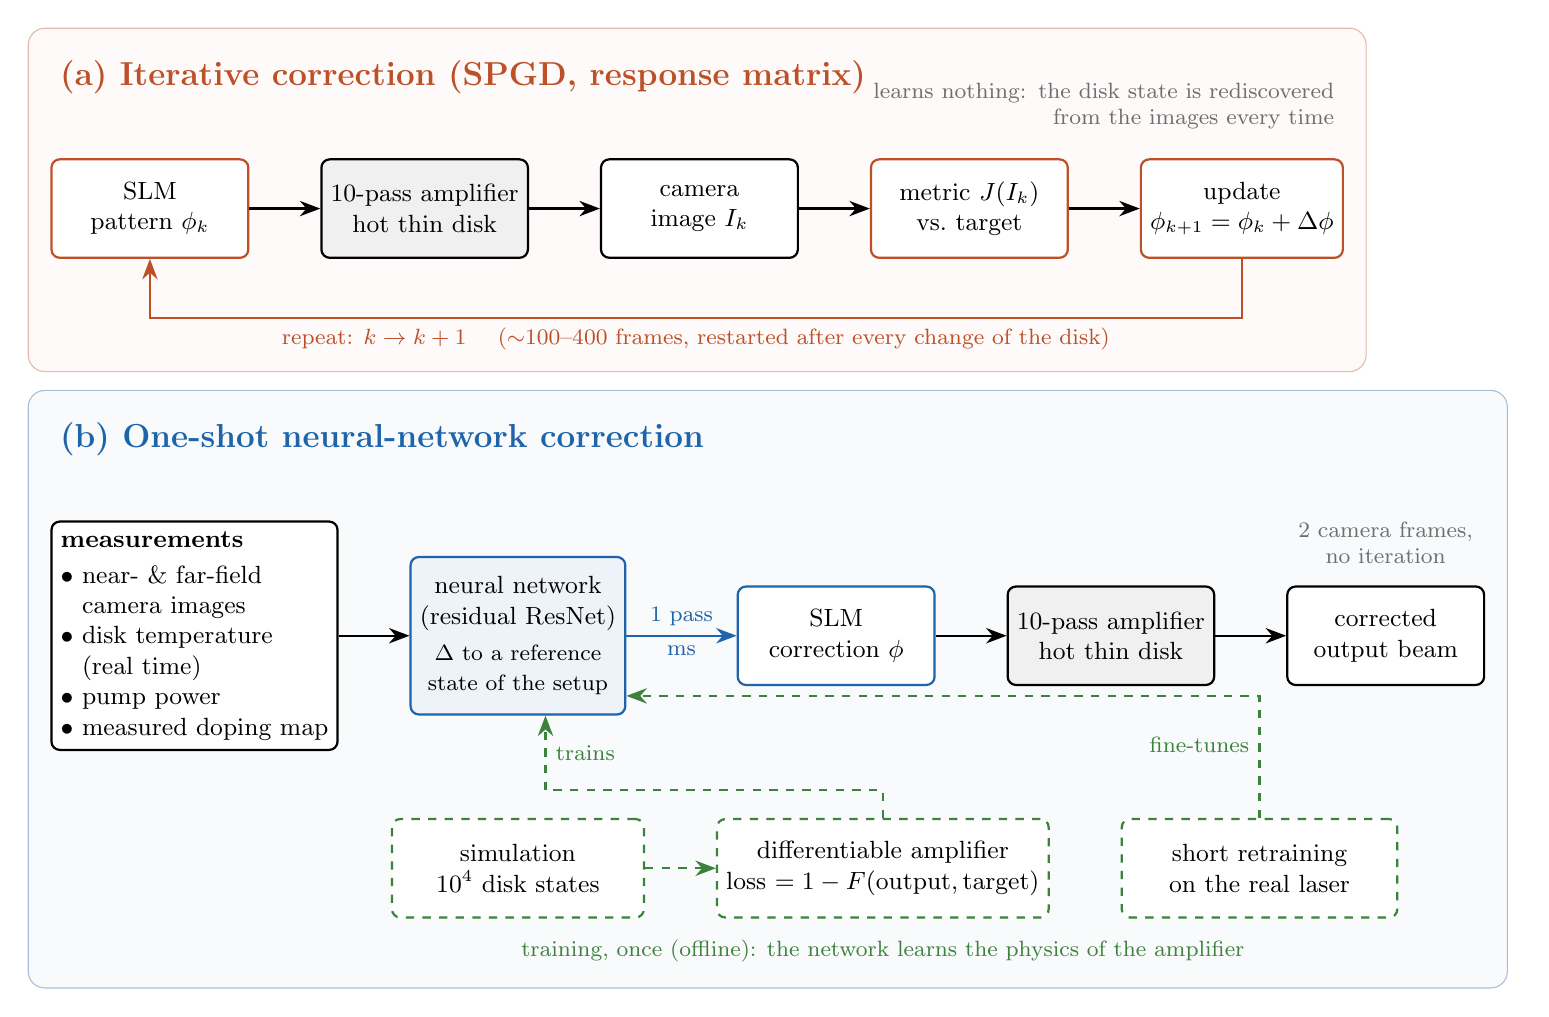
\begin{tikzpicture}[node distance=0.8cm and 0.9cm]

% ----------------------------------------------------------------------------------------------------
% (a) iterative correction
% ----------------------------------------------------------------------------------------------------
\node[title, text=iter] (ta) at (0, 0) {(a) Iterative correction (SPGD, response matrix)};

\node[box, draw=iter, below=0.7cm of ta.south west, anchor=north west] (slmA) {SLM\\pattern $\phi_k$};
\node[laser, right=of slmA] (ampA) {10-pass amplifier\\hot thin disk};
\node[box, right=of ampA] (camA) {camera\\image $I_k$};
\node[box, draw=iter, right=of camA] (metA) {metric $J(I_k)$\\vs.\ target};
\node[box, draw=iter, right=of metA] (updA) {update\\$\phi_{k+1}=\phi_k+\Delta\phi$};

\draw[arr] (slmA) -- (ampA);
\draw[arr] (ampA) -- (camA);
\draw[arr] (camA) -- (metA);
\draw[arr] (metA) -- (updA);
\draw[arr, iter] (updA.south) -- ++(0, -0.75) -| node[pos=0.25, below, font=\footnotesize] {repeat: $k \to k+1$ \quad ($\sim$100--400 frames, restarted after every change of the disk)} (slmA.south);

\node[note, above=0.25cm of updA.north east, anchor=south east, text width=6cm, align=right] (noteA) {learns nothing: the disk state is rediscovered\\from the images every time};

% ----------------------------------------------------------------------------------------------------
% (b) one-shot network
% ----------------------------------------------------------------------------------------------------
\node[title, text=nn] (tb) at (0, -4.6) {(b) One-shot neural-network correction};

\node[box, below=0.7cm of tb.south west, anchor=north west, minimum width=3.1cm, minimum height=2.9cm, align=left] (inB)
  {\textbf{measurements}\\[2pt]
   $\bullet$ near- \& far-field\\\phantom{$\bullet$} camera images\\
   $\bullet$ disk temperature\\\phantom{$\bullet$} (real time)\\
   $\bullet$ pump power\\
   $\bullet$ measured doping map};
\node[box, draw=nn, fill=nn!8, right=of inB, minimum height=2.0cm] (net) {neural network\\(residual ResNet)\\[2pt]\footnotesize $\Delta$ to a reference\\\footnotesize state of the setup};
\node[box, draw=nn, right=1.4cm of net] (slmB) {SLM\\correction $\phi$};
\node[laser, right=of slmB] (ampB) {10-pass amplifier\\hot thin disk};
\node[box, right=of ampB] (outB) {corrected\\output beam};

\draw[arr] (inB) -- (net);
\draw[arr, nn] (net) -- node[above, font=\footnotesize] {1 pass} node[below, font=\footnotesize] {ms} (slmB);
\draw[arr] (slmB) -- (ampB);
\draw[arr] (ampB) -- (outB);

\node[note, above=0.15cm of outB, text width=3.2cm] {2 camera frames,\\no iteration};

% training (offline)
\node[box, draw=phys, dashed, below=1.3cm of net, minimum width=3.2cm] (sim) {simulation\\10$^4$ disk states};
\node[box, draw=phys, dashed, right=of sim, minimum width=4.2cm] (loss) {differentiable amplifier\\loss $= 1-F(\text{output}, \text{target})$};
\node[box, draw=phys, dashed, right=of loss, minimum width=3.5cm] (lab) {short retraining\\on the real laser};

\draw[arr, phys, dashed] (sim) -- (loss);
\draw[arr, phys, dashed] (loss.north) -- ++(0, 0.35) -| node[pos=0.75, right, font=\footnotesize] {trains} ($(net.south)+(0.35,0)$);
\draw[arr, phys, dashed] (lab.north) |- node[pos=0.3, left, font=\footnotesize] {fine-tunes} ($(net.south east)+(0,0.25)$);
\node[note, below=0.15cm of loss, text=phys] {training, once (offline): the network learns the physics of the amplifier};

\coordinate (endA) at ($(slmA.south)+(0,-1.15)$);
\coordinate (endB) at ($(loss.south)+(0,-0.6)$);
\begin{scope}[on background layer]
  \node[draw=iter!40, rounded corners=6pt, fill=iter!3, inner sep=8pt, fit=(ta) (slmA) (updA) (endA) (noteA)] {};
  \node[draw=nn!40, rounded corners=6pt, fill=nn!3, inner sep=8pt, fit=(tb) (inB) (outB) (sim) (lab) (endB)] {};
\end{scope}
\end{tikzpicture}
\end{document}
